\documentclass[a4paper,11pt]{article}
\usepackage[utf8]{inputenc}\usepackage[T1]{fontenc}
\usepackage[english]{babel}\usepackage{lmodern}\usepackage{microtype}
\usepackage{amsmath,amssymb}\usepackage{geometry}
\geometry{a4paper,left=2.2cm,right=2.2cm,top=2.0cm,bottom=2.0cm}
\usepackage{booktabs,array}\usepackage{xcolor}
\definecolor{bokug}{RGB}{0,135,60}\usepackage{tikz}
\usetikzlibrary{arrows.meta,calc}
\usepackage{fancyhdr}\pagestyle{fancy}
\renewcommand{\headrulewidth}{0.4pt}
\usepackage{enumitem}\setlength{\parindent}{0pt}\setlength{\parskip}{4pt}

\begin{document}
\fancyhead[L]{\small VU Mechanik – LAWI 100515 (PI)}\fancyhead[R]{\small SS 2026}\fancyfoot[C]{\thepage}
\begin{center}{\large\bfseries\color{bokug}University of Natural Resources and Life Sciences, Vienna (BOKU)}\\[2pt]{\large\bfseries VU Mechanik – LAWI 100515 (PI)}\\[4pt]Exam \textbf{Group A} \hfill Date: 26.06.2026\\[2pt]\rule{\linewidth}{0.4pt}\end{center}

\begin{center}\textbf{\large Model solution}\end{center}
\begin{center}
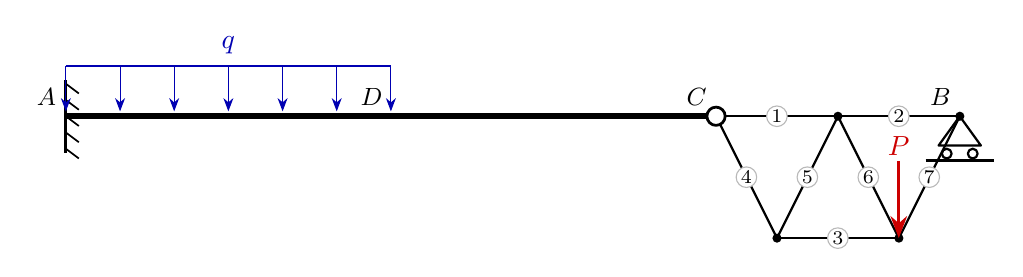
\begin{tikzpicture}[scale=1.032,>=Stealth,line join=round]
  \coordinate (P0) at (0.000,0.000);
  \coordinate (P1) at (4.000,0.000);
  \coordinate (P2) at (8.000,0.000);
  \coordinate (TO1) at (9.500,0.000);
  \coordinate (TO2) at (11.000,0.000);
  \coordinate (TU0) at (8.750,-1.500);
  \coordinate (TU1) at (10.250,-1.500);
  \draw[thick] (P2) -- (TO1);
  \draw[thick] (TO1) -- (TO2);
  \draw[thick] (TU0) -- (TU1);
  \draw[thick] (P2) -- (TU0);
  \draw[thick] (TU0) -- (TO1);
  \draw[thick] (TO1) -- (TU1);
  \draw[thick] (TU1) -- (TO2);
  \draw[line width=2.2pt] (P0) -- (P1);
  \draw[line width=2.2pt] (P1) -- (P2);
  \fill (P2) circle (1.6pt);
  \fill (TO1) circle (1.6pt);
  \fill (TO2) circle (1.6pt);
  \fill (TU0) circle (1.6pt);
  \fill (TU1) circle (1.6pt);
  \draw[fill=white,line width=1pt] (P2) circle (3.2pt);
  \draw[line width=1.1pt] (0.000,-0.450) -- (0.000,0.450);
  \draw[line width=0.6pt] (0.000,-0.400) -- (0.160,-0.520);
  \draw[line width=0.6pt] (0.000,-0.200) -- (0.160,-0.320);
  \draw[line width=0.6pt] (0.000,0.000) -- (0.160,-0.120);
  \draw[line width=0.6pt] (0.000,0.200) -- (0.160,0.080);
  \draw[line width=0.6pt] (0.000,0.400) -- (0.160,0.280);
  \draw[thick] (11.000,0.000) -- (10.740,-0.360) -- (11.260,-0.360) -- cycle;
  \draw[thick] (10.840,-0.460) circle (0.06) (11.160,-0.460) circle (0.06);
  \draw[line width=1pt] (10.580,-0.540) -- (11.420,-0.540);
  \node[circle,fill=white,draw=gray!55,inner sep=0.5pt,font=\scriptsize] at (8.750,0.000) {1};
  \node[circle,fill=white,draw=gray!55,inner sep=0.5pt,font=\scriptsize] at (10.250,0.000) {2};
  \node[circle,fill=white,draw=gray!55,inner sep=0.5pt,font=\scriptsize] at (9.500,-1.500) {3};
  \node[circle,fill=white,draw=gray!55,inner sep=0.5pt,font=\scriptsize] at (8.375,-0.750) {4};
  \node[circle,fill=white,draw=gray!55,inner sep=0.5pt,font=\scriptsize] at (9.125,-0.750) {5};
  \node[circle,fill=white,draw=gray!55,inner sep=0.5pt,font=\scriptsize] at (9.875,-0.750) {6};
  \node[circle,fill=white,draw=gray!55,inner sep=0.5pt,font=\scriptsize] at (10.625,-0.750) {7};
  \draw[->,blue!70!black] (0.000,0.620) -- (0.000,0.060);
  \draw[->,blue!70!black] (0.667,0.620) -- (0.667,0.060);
  \draw[->,blue!70!black] (1.333,0.620) -- (1.333,0.060);
  \draw[->,blue!70!black] (2.000,0.620) -- (2.000,0.060);
  \draw[->,blue!70!black] (2.667,0.620) -- (2.667,0.060);
  \draw[->,blue!70!black] (3.333,0.620) -- (3.333,0.060);
  \draw[->,blue!70!black] (4.000,0.620) -- (4.000,0.060);
  \draw[blue!70!black,thick] (0.000,0.620) -- (4.000,0.620);
  \node[blue!70!black] at (2.000,0.870) {$q$};
  \draw[->,red!80!black,line width=1.1pt] (10.250,-0.550) -- (10.250,-1.500);
  \node[red!80!black] at (10.250,-0.370) {$P$};
  \node[font=\small] at (0.000,0.000) [xshift=-7pt,yshift=7pt] {$A$};
  \node[font=\small] at (4.000,0.000) [xshift=-7pt,yshift=7pt] {$D$};
  \node[font=\small] at (8.000,0.000) [xshift=-7pt,yshift=7pt] {$C$};
  \node[font=\small] at (11.000,0.000) [xshift=-7pt,yshift=7pt] {$B$};
\end{tikzpicture}
\end{center}
\par\medskip\textbf{1.\ Static determinacy}\par Counting criterion $n=3k-(a+z)$ (bodies $k$, reactions $a$, interaction forces $z$):
\[ n=3k-(a+z)=3\cdot2-(4+2)=0\ \Rightarrow\ \text{statically determinate} \]
\par\medskip\textbf{2.\ Support reactions and hinge forces}\par
$A:\ R_x=0,\ R_y=18.5,\ M=52$\quad $B:\ R_x=0,\ R_y=7.5$\par $C:\ H_x=0,\ H_y=-2.5$
\par\medskip\textbf{3.\ Truss member forces}\par
\begin{center}\renewcommand{\arraystretch}{1.1}\begin{tabular}{c r l}
\toprule
Member & Force $S$ [kN] & Type \\
\midrule
  1 & -1.25 & compression \\
  2 & -3.75 & compression \\
  3 & 2.5 & tension \\
  4 & 2.8 & tension \\
  5 & -2.8 & compression \\
  6 & 2.8 & tension \\
  7 & 8.39 & tension \\
\bottomrule
\end{tabular}\end{center}
\begin{center}
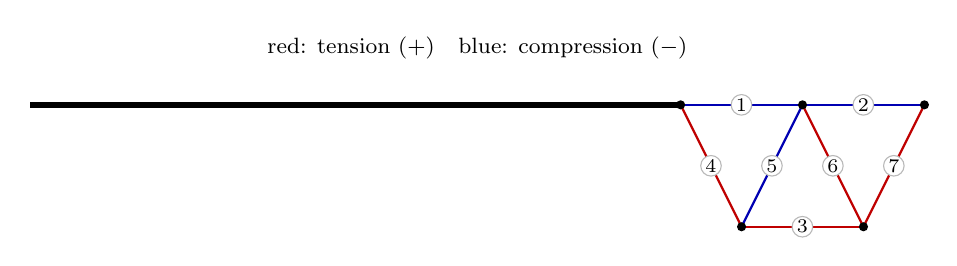
\begin{tikzpicture}[scale=1.032,>=Stealth,line join=round]
  \coordinate (P0) at (0.000,0.000);
  \coordinate (P1) at (4.000,0.000);
  \coordinate (P2) at (8.000,0.000);
  \coordinate (TO1) at (9.500,0.000);
  \coordinate (TO2) at (11.000,0.000);
  \coordinate (TU0) at (8.750,-1.500);
  \coordinate (TU1) at (10.250,-1.500);
  \draw[thick,blue!70!black] (P2) -- (TO1);
  \draw[thick,blue!70!black] (TO1) -- (TO2);
  \draw[thick,red!75!black] (TU0) -- (TU1);
  \draw[thick,red!75!black] (P2) -- (TU0);
  \draw[thick,blue!70!black] (TU0) -- (TO1);
  \draw[thick,red!75!black] (TO1) -- (TU1);
  \draw[thick,red!75!black] (TU1) -- (TO2);
  \draw[line width=2pt] (P0) -- (P1);
  \draw[line width=2pt] (P1) -- (P2);
  \fill (P2) circle (1.6pt);
  \fill (TO1) circle (1.6pt);
  \fill (TO2) circle (1.6pt);
  \fill (TU0) circle (1.6pt);
  \fill (TU1) circle (1.6pt);
  \node[circle,fill=white,draw=gray!55,inner sep=0.5pt,font=\scriptsize] at (8.750,0.000) {1};
  \node[circle,fill=white,draw=gray!55,inner sep=0.5pt,font=\scriptsize] at (10.250,0.000) {2};
  \node[circle,fill=white,draw=gray!55,inner sep=0.5pt,font=\scriptsize] at (9.500,-1.500) {3};
  \node[circle,fill=white,draw=gray!55,inner sep=0.5pt,font=\scriptsize] at (8.375,-0.750) {4};
  \node[circle,fill=white,draw=gray!55,inner sep=0.5pt,font=\scriptsize] at (9.125,-0.750) {5};
  \node[circle,fill=white,draw=gray!55,inner sep=0.5pt,font=\scriptsize] at (9.875,-0.750) {6};
  \node[circle,fill=white,draw=gray!55,inner sep=0.5pt,font=\scriptsize] at (10.625,-0.750) {7};
  \node[font=\footnotesize] at (5.50,0.70) {red: tension $(+)$\quad blue: compression $(-)$};
\end{tikzpicture}
\end{center}
\par\medskip\textbf{4.\ Section-force diagrams of the beams}\par
\begin{center}
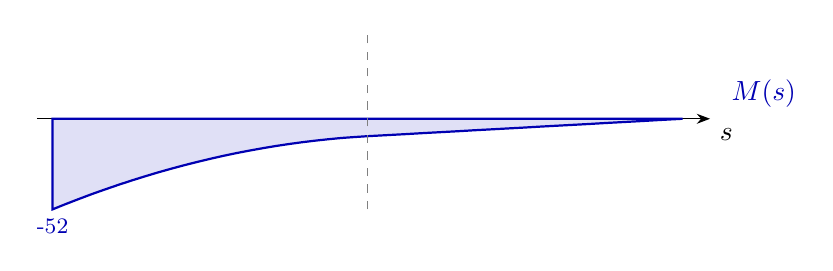
\begin{tikzpicture}[>=Stealth]
  \draw[->] (-0.2,0) -- (8.35,0) node[below right]{$s$};
  \filldraw[fill=blue!70!black!12,draw=blue!70!black,thick] (0,0) -- plot coordinates {(0.000,-1.150) (0.167,-1.083) (0.333,-1.019) (0.500,-0.956) (0.667,-0.897) (0.833,-0.840) (1.000,-0.785) (1.167,-0.733) (1.333,-0.683) (1.500,-0.636) (1.667,-0.591) (1.833,-0.549) (2.000,-0.509) (2.167,-0.471) (2.333,-0.436) (2.500,-0.404) (2.667,-0.374) (2.833,-0.346) (3.000,-0.321) (3.167,-0.298) (3.333,-0.278) (3.500,-0.260) (3.667,-0.244) (3.833,-0.232) (4.000,-0.221) (4.000,-0.221) (4.167,-0.212) (4.333,-0.203) (4.500,-0.194) (4.667,-0.184) (4.833,-0.175) (5.000,-0.166) (5.167,-0.157) (5.333,-0.147) (5.500,-0.138) (5.667,-0.129) (5.833,-0.120) (6.000,-0.111) (6.167,-0.101) (6.333,-0.092) (6.500,-0.083) (6.667,-0.074) (6.833,-0.065) (7.000,-0.055) (7.167,-0.046) (7.333,-0.037) (7.500,-0.028) (7.667,-0.018) (7.833,-0.009) (8.000,0.000)} -- (8.000,0) -- cycle;
  \draw[gray,dashed,thin] (4.000,-1.15) -- (4.000,1.15);
  \node[below,blue!70!black,font=\footnotesize] at (0.000,-1.150) {-52};
  \node[blue!70!black,right] at (8.50,0.32) {$M(s)$};
\end{tikzpicture}\\[5pt]
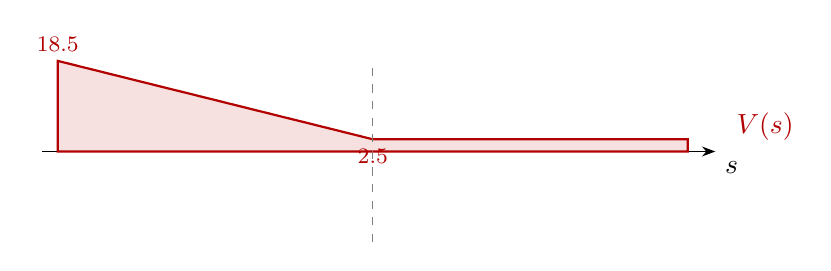
\begin{tikzpicture}[>=Stealth]
  \draw[->] (-0.2,0) -- (8.35,0) node[below right]{$s$};
  \filldraw[fill=red!70!black!12,draw=red!70!black,thick] (0,0) -- plot coordinates {(0.000,1.150) (0.167,1.109) (0.333,1.067) (0.500,1.026) (0.667,0.984) (0.833,0.943) (1.000,0.901) (1.167,0.860) (1.333,0.818) (1.500,0.777) (1.667,0.736) (1.833,0.694) (2.000,0.653) (2.167,0.611) (2.333,0.570) (2.500,0.528) (2.667,0.487) (2.833,0.445) (3.000,0.404) (3.167,0.363) (3.333,0.321) (3.500,0.280) (3.667,0.238) (3.833,0.197) (4.000,0.155) (4.000,0.155) (4.167,0.155) (4.333,0.155) (4.500,0.155) (4.667,0.155) (4.833,0.155) (5.000,0.155) (5.167,0.155) (5.333,0.155) (5.500,0.155) (5.667,0.155) (5.833,0.155) (6.000,0.155) (6.167,0.155) (6.333,0.155) (6.500,0.155) (6.667,0.155) (6.833,0.155) (7.000,0.155) (7.167,0.155) (7.333,0.155) (7.500,0.155) (7.667,0.155) (7.833,0.155) (8.000,0.155)} -- (8.000,0) -- cycle;
  \draw[gray,dashed,thin] (4.000,-1.15) -- (4.000,1.15);
  \node[above,red!70!black,font=\footnotesize] at (0.000,1.150) {18.5};
  \node[below,red!70!black,font=\footnotesize] at (4.000,0.155) {2.5};
  \node[red!70!black,right] at (8.50,0.32) {$V(s)$};
\end{tikzpicture}\\[5pt]
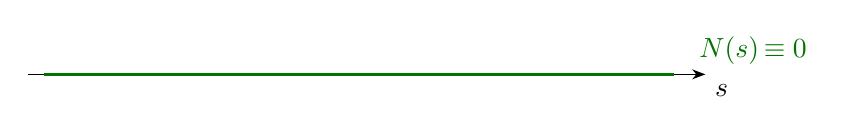
\begin{tikzpicture}[>=Stealth]
  \draw[->] (-0.2,0) -- (8.40,0) node[below right]{$s$};
  \draw[green!45!black,very thick] (0,0) -- (8,0);
  \node[green!45!black,right] at (8.2,0.3) {$N(s)$\,$\equiv 0$};
\end{tikzpicture}\\[10pt]
\end{center}
\end{document}